\documentclass[12pt,a4paper]{article}

\usepackage[utf8]{inputenc}
\usepackage[a4paper,total={150mm,240mm}]{geometry}
\usepackage[american]{babel}

\usepackage{float}
\usepackage{babel}
\usepackage{amsmath}
\usepackage{tikz}
\usepackage{graphicx}
\usepackage{amssymb}
\usepackage{tikz}

\usepackage{listings}
\definecolor{listingbg}{gray}{0.95}
\lstset{
  language=c++,
  basicstyle=\ttfamily\small,
  frame=single,
  backgroundcolor=\color{listingbg},
  breaklines=true,
  postbreak=\raisebox{0ex}[0ex][0ex]{\ensuremath{\color{red}\hookrightarrow\space}}
}

\usepackage{stmaryrd}
\newcommand\jump[1]{\llbracket #1 \rrbracket}
\newcommand\avg[1]{\{ #1 \}}
\newcommand\avgw[1]{\{ #1 \}_{\omega}}
\newcommand{\vx}{\vec x}
\newcommand{\grad}{\vec \nabla}
\newcommand{\wind}{\vec \beta}
\newcommand{\Laplace}{\Delta}
\newcommand{\mycomment}[1]{}

%% Typesetting C++
\def\CC{{C\nolinebreak[4]\hspace{-.05em}\raisebox{.4ex}{\tiny\bf ++}}}

% Exercise stylesheet
\usepackage{exercise}

\title{\textbf{Exercises for Tutorial09}}
\subtitle{Generating Local Operators}
\exerciselabel{Exercise}

\begin{document}

\exerciseheader

In tutorial09 we learned how to use the \lstinline{dune-codegen} module to
generate local operators. In this exercise we will use this to generate some
more complicated discretizations.

The build directory of this exercise is
\begin{lstlisting}
dune-course/release-build/dune-pdelab-tutorials/tutorial09/exercise/task
\end{lstlisting}

The corresponding source directory can be found under
\begin{lstlisting}
dune-course/dune/dune-pdelab-tutorials/tutorial09/exercise/task
\end{lstlisting}
or by following the symlink in the build directory
\begin{lstlisting}
dune-course/release-build/dune-pdelab-tutorials/tutorial09/exercise/task/src_dir
\end{lstlisting}


\begin{Exercise}{Navier Stokes}
  In this exercise we will implement the Navier Stokes equations for a flow
  around a cylinder\footnote{See
    http://www.featflow.de/en/benchmarks/cfdbenchmarking/flow/dfg\_benchmark2\_re100.html
    for a more detailed benchmark description} on the two dimenisional domain
  $\Omega$ shown below and the time interval $\Sigma$.

  \begin{equation}
    \begin{aligned}
      \rho \partial_t \vec{u} - \nu \Laplace \vec{u} + \rho (\nabla \vec{u}) \vec{u} + \nabla p &= 0 \qquad \text{in $\Omega$}\\
      \nabla \cdot \vec{u} &= 0 \qquad \text{in $\Omega$}
    \end{aligned}
    \label{eq:navier-stokes}
  \end{equation}

  Here $\vec{u}:\Omega\times\Sigma\to\mathbb{R}^2$ is the unknown velocity
  field and $p:\Omega\times\Sigma\to\mathbb{R}$ is the unknown pressure. We
  assume that the kinematic viscosity $\nu=0.001$ and the fluid density
  $\rho=1$ are constant. The domain $\Omega$ is a rectangle with a circular
  hole.

  \begin{center}
    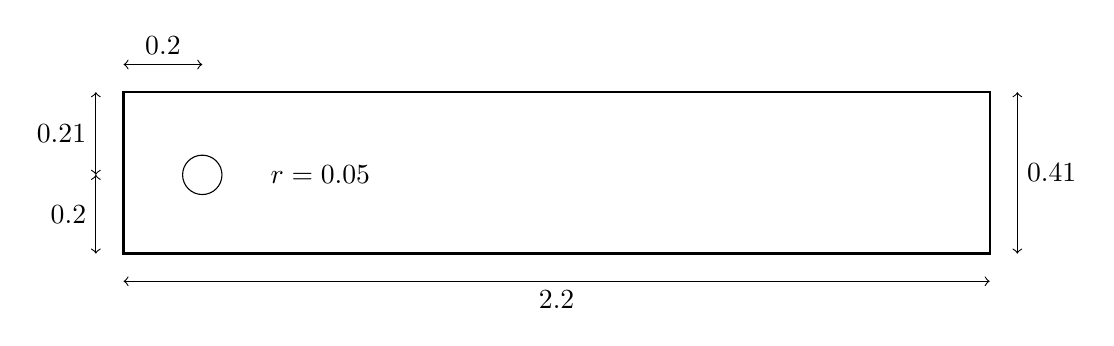
\begin{tikzpicture}[scale=5]
      \coordinate (a) at (0,0);
      \coordinate (b) at (2.2,0);
      \coordinate (c) at (2.2,0.41);
      \coordinate (d) at (0,0.41);

      \coordinate (e) at (0,0.2);
      \coordinate (f) at (0.2,0.41);


      \draw[thick] (a) -- (b) -- (c) -- (d) --cycle;
      \draw (0.2,0.2) circle (0.05);

      \draw[<->] ([yshift=-2]a) -- ([yshift=-2]b) node[midway, below]{2.2};
      \draw[<->] ([xshift=2]b) -- ([xshift=2]c) node[midway, right]{0.41};

      \draw[<->] ([xshift=-2]a) -- ([xshift=-2]e) node[midway, left]{0.2};
      \draw[<->] ([xshift=-2]e) -- ([xshift=-2]d) node[midway, left]{0.21};
      \draw[<->] ([yshift=2]d) -- ([yshift=2]f) node[midway, above]{0.2};

      \node at (0.5,0.2) {$r=0.05$};
    \end{tikzpicture}
  \end{center}

  As boundary conditions we use
  \begin{align*}
    \vec{u} &= 0 && \text{on $\partial\Omega \cap (0,2.2)\times[0,0.41]$} \\
    \vec{u} &=
    \begin{pmatrix}
      1.5 \cdot 4 \cdot x_1 \frac{0.41-x_1}{0.41^2} \cdot s(t) \\ 0
    \end{pmatrix} && \text{on $0\times[0,0.41]$}\\
    \nu \, \nabla \vec{u} \, \vec{n} - p\vec{n} &= 0 && \text{on $2.2\times[0,0.41]$}
  \end{align*}
  with the function
  \begin{equation*}
    s(t) =
    \begin{cases}
      \sin\left(\frac{\pi t}{8}\right) \qquad &\text{if $t<4$}\\
      1 \qquad &\text{else}
    \end{cases}
  \end{equation*}
  The initial conditions are simply
  \begin{align*}
    \vec{u}|_{t=0} &= 0 \\
    p|_{t=0} &= 0. \\
  \end{align*}

  A semi-discretization in space of this equation is: Find
  $(\vec{u}_h,p_h) \in U_h\times Q_h$ with
  \begin{equation*}
    \rho (\partial_t \vec{u}_h, \vec{v}_h)_\Omega + r_h(\vec{u}_h, p_h, \vec{v}_h, q_h) = 0 \qquad \forall (\vec{v}_h,q_h) \in V_h\times Q_h
  \end{equation*}
  for appropriate function spaces $U_h$, $V_h$, $Q_h$ and residual
  \begin{equation}
    r_h(\vec{u},p,\vec{v},q)
    = \nu (\nabla \vec{u}, \nabla \vec{v})_{0,\Omega}
    - (p, \nabla \cdot \vec{v})_{0,\Omega}
    - (q, \nabla \cdot \vec{u})_{0, \Omega}
    + \rho ((\nabla \vec{u}) \vec{u}, \vec{v})_{0, \Omega}
    \label{eq:ns-residual}
  \end{equation}

  Go to the source directory of this exercise. There you will find the files
  \lstinline{navier_stokes.ufl} and \lstinline{navier_stokes.ini}. Open the UFL
  file and implement the correct residual for the spatial discretization and
  the correct boundary conditions. For generating the \CC\ file and compiling
  go to the build directory and type
  \begin{lstlisting}
make navier_stokes
  \end{lstlisting}

  Help:
  \begin{itemize}
  \item UFL has a conditional:
    \begin{displaymath}
      \text{\lstinline{conditional(cond, A, B)}} = \left\{
        \begin{array}{lr}
          \text{\lstinline{A}} & \text{\lstinline{cond is True}} \\
          \text{\lstinline{B}} & \text{\lstinline{cond is False}}
        \end{array}
      \right.
    \end{displaymath}
  \item UFL has \lstinline{grad(.)} and \lstinline{div(.)}
  \item \lstinline{inner(.,.)*dx} will do the right thing for all scalar
    products of equation \eqref{eq:ns-residual}. Just make sure that the
    dimensions of the two arguments match.
  \item UFL has a method \lstinline{sin(.)}.
  \end{itemize}
\end{Exercise}

\begin{Exercise}{Nonlinear Poisson with Discontinuous Galerkin Method}
  In this exercise we will solve the nonlinear Poisson equation
  \begin{equation}
    \begin{aligned}
      -\Delta u + q(u) &= f &&\text{in $\Omega$},\\
      u &= g &&\text{on $\partial\Omega$}
    \end{aligned}
    \label{eq:nonlinear_poisson}
  \end{equation}

  with the nonlinear function $q(u)=\eta u^2$ and the parameters functions
  \begin{align*}
    g(x) = \|x\|_2^2 \\
    f(x) = -2 d + \eta \, g(x)^2
  \end{align*}
  using the discontinuous Galerkin (DG) method. In our case the dimension $d$
  is two and the parameter $\eta$ describes the strength of the
  nonlinearity. You can for example set $\eta=2$. We will focus on the
  implementation of this method in UFL to show the power of this approach
  without going into details about the numerical method.\footnote{For further
    insight into DG methods see e.g. Di Pietro, Daniele Antonio and Ern,
    Alexandre: Mathematical aspects of discontinuous Galerkin methods}

  In contrast to continuous Galerkin methods DG methods use piecewise
  polynomial basis functions on the grid and allow for discontinuities along
  faces. In order to get a discritzation that still approximates the solution
  of our PDE penalty terms along the faces are introduced. Dirichlet boundary
  conditions are not build into the ansatz space but enforced in a weak way
  like it was done in exercise01 using Nitsche boundary condition.

  A\footnote{There are different DG discretizations. We use symmetric interior penalty here.} DG discretization of problem \eqref{eq:nonlinear_poisson} reads the
  following: Find $u_h$ in $U_h$ with
  \begin{equation*}
    r_h(u_h, v_h) = 0 \qquad \forall v_h \in V_h
  \end{equation*}
  with the residual
  \begin{equation}
    \label{eq:nonlinear_poisson_dg}
    \begin{aligned}
      r_h(u, v) & = \sum_{T\in\mathcal{T}_h}\int_T \nabla u\cdot\nabla v + q(u)v - fv\ dx\\
      &\quad - \sum_{F\in\mathcal{F}_h}\int_F (\avg{\nabla u}, \vec{n})\jump{v} + \jump{u}(\avg{\nabla v}, \vec{n}) - \gamma_F\jump{u}\jump{v}\ ds\\
      &\quad - \sum_{F\in\mathcal{B}_h}\int_F(\nabla u, \vec{n})v + (u-g)(\nabla v, \vec{n}) - \gamma_F(u-g)v\ ds
    \end{aligned}
  \end{equation}

  We need to explain some notation: \footnote{For faces we sometimes refer to the inner or the outer cell. For a given face it doesn't matter which cell is the inner and which is the outer as long as it is always treated the same for this face. This is not important for this exercise.}

  \begin{itemize}
  \item $\mathcal{T}_h$: Set of mesh elements. Use \lstinline{...*dx} in the
    UFL file for volume integrals. You don't need to care about the sum in
    front of the integral. UFL describes only the local integrals and will do
    the right thing.
  \item $\mathcal{B}_h$: Set of boundary faces. Use \lstinline{...*ds} in the
    UFL file for integrals over boundary faces.
  \item $\mathcal{F}_h$: Set of inner faces. Use \lstinline{...*dS} in the UFL
    file for integrals over inner faces.
  \item $\vec{n}$: Unit outer normal vector pointing from the inner cell to the
    outer cell. In the UFL file use \lstinline{n = FacetNormal(cell)('+')}
  \item $\avg{.}$: Average of the values at the inside cell and the outside
    cell. Only makes sense at faces. In the UFL file use \lstinline{avg(.)}.
  \item $\jump{.}$: Value at the inside cell minus value at the outside
    cell. Only makes sense at faces. In the UFL file use \lstinline{jump(.)}.
  \item $\gamma_F$: Penalty parameter of the DG scheme. For this exercise we
    just choose $\gamma_F = 100$. A good choice of $\gamma_F$ depends on the
    dimension, degree of your discretization and geometry informations. See the
    book mentioned above for further detail.
  \end{itemize}

  After reading all this text we can finally start doing some work:
  \begin{enumerate}
  \item Go to the source directory of this exercise. There you can find the
    files \lstinline{nonlinear_poisson_dg.ufl} and
    \lstinline{nonlinear_poisson_dg.mini} and a target is defined in the
    \lstinline{CMakeLists.txt} file.
  \item You need to implement the residual \eqref{eq:nonlinear_poisson_dg} in
    the UFL file.
  \end{enumerate}

\end{Exercise}

\end{document}
